\subsection{ Methodology}

GANs are generative models that learn a mapping from random noise vector z to output image y, G : z → y. In 

	\begin{figure}[h!]
     \centering
    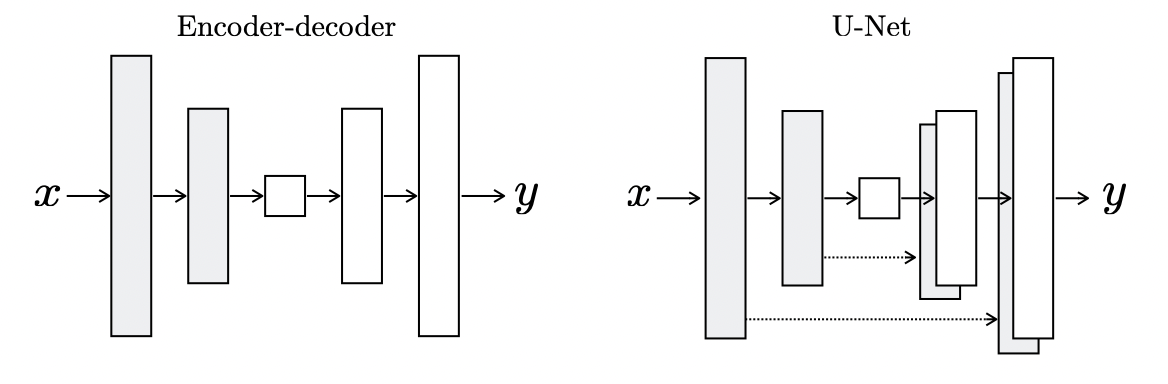
\includegraphics[width=\linewidth,height=7cm]{figures/5.png}
    \caption{ Two choices for the architecture of the generator. The “U-Net” is an encoder-decoder with skip connections between mirrored layers in the encoder and decoder stacks }
    \label{fig:GAN model}

\end{figure}

\subsection{Network architectures}

The architectures of our generator and discriminator are based on those in. Convolution-BatchNorm-ReLu modules are used by both the generator and the discriminator.

\subsection{Generator with skips}

The mapping of a high resolution input grid to a high resolution output grid is a distinguishing property of image-to-image translation difficulties. Furthermore, the input and output for the problems we analyse have different surface appearances, but they are both renderings of the same underlying structure. As a result, the input structure is closely aligned with the output structure. The generator architecture is based on these concepts.

\par An encoder-decoder network has been employed in several past solutions to difficulties in this field. The input is transmitted through a series of layers that gradually downsample the data until it reaches a bottleneck layer, when the process is reversed. All information flow must pass through all layers, including the bottleneck, in such a network. There is a lot of low-level information shared between the input and output for many picture translation difficulties, and it would be preferable to send this information directly across the network. In image colorization, for example, the input and output share the location of prominent edges.


\par We add skip connections, which follow the general shape of a "U-Net," to provide the generator a way to get around the bottleneck for information like this. We add skip connections between each layer I and layer n I where n is the total number of layers, in particular. Each skip connection simply concatenates all layer I channels with layer n-i channels.

\subsection{Markovian discriminator (PatchGAN)}

On image production challenges, it is generally known that the L2 loss and L1 generate hazy outcomes. Although these losses may not promote high-frequency sharpness, they do, in many circumstances, accurately capture low frequencies. We don't need a totally new system to enforce accuracy at low frequencies for cases when this is the case. L1 is sufficient.

This justifies using an L1 term to force low-frequency accuracy by confining the GAN discriminator to exclusively simulate high-frequency structure. It is sufficient to limit our attention to the structure in local image patches in order to represent high-frequencies. As a result, we create a PatchGAN, a discriminator architecture that only penalises structure at the patch size. This discriminator attempts to determine whether each of an image's N N patches is authentic or phoney. We convolutionally run this discriminator across the image, average all responses to get the final output of D.

We show that N can be substantially smaller than the image's full size while still producing high-quality results. This is beneficial since a smaller PatchGAN has less parameters, runs faster, and can process images of any size.
A discriminator like this effectively represents the image as a Markov random field, assuming that pixels separated by more than a patch diameter are independent. This link was previously investigated in, and it is also a prevalent assumption in texture and style models. As a result, our PatchGAN can be viewed as a texture/style loss.

\subsection{Optimization and inference}

\par We use the traditional strategy of alternating between one gradient descent step on D and one step on G to improve our networks. Rather than training G to minimise log(1 D(x, G(x, z)), we train it to maximise log D(x, G(x, z) as indicated in the original GAN study. In addition, we divide the goal by two while optimising D, which reduces D's learning rate compared to G's. With a learning rate of 0.0002, and momentum parameters 1 = 0.5, 2 = 0.999, we employ minibatch SGD and the Adam solver.

\par At inference time, we run the generator net in the same way that we did during training. This differs from the standard technique in that we apply dropout at test time and batch normalisation using the test batch's statistics rather than the training batch's aggregated data. When the batch size is set to 1, this method of batch normalising is known as "instance normalisation," and it has been shown to be effective in picture production jobs. Depending on the experiment, we utilise batch sizes ranging from one to ten.